\documentclass[notitlepage, twocolumn,11pt]{article}
\usepackage{fullpage}
\usepackage[affil-it]{authblk}
\usepackage{hyperref}
\usepackage{graphicx}
\usepackage[backend=bibtex, style=numeric]{biblatex}

\addbibresource{report.bib}

\makeatletter
\def\blfootnote{\gdef\@thefnmark{}\@footnotetext}
\makeatother

\title{\bf
Program 2\\
The Way the \textit{Disk} turns
}

\date{November 2015}
\author{
Matt McCarthy
}
\affil{Christopher Newport University\\
\textbf{CPSC 621 Parallel Processing}\\
\texttt{\href{mailto:matthew.mccarthy.12@cnu.edu}{matthew.mccarthy.12@cnu.edu}}
}


\begin{document}

\nocite{*}

\maketitle

\noindent\textbf{Abstract}

\noindent We investigate the effect of spatial and temporal locality on disk I/O and cache performance.
\blfootnote{Source can be found at \url{https://github.com/matt-mccarthy/verdant-octo-kumquat}.}

\section{Background}

In order to parallelize code, a developer must first decide how to decompose the problem.
A common and simple decomposition is data decomposition where the developer assigns different blocks of data to each processor.
However, when the data is stored on a disk, like in a database scenario, I/O performance becomes a significant bottleneck.
While the operating system has primary responsibility for optimizing disk reads, it only has a small number of read requests with which it can make decisions on how to optimally move the disk arm.
Thus, when possible, the developer should endeavor to use spatial and temporal locality at the application level.

\section{Set up}

We consider a file system containing 2GB of text files, each of which is exactly 14KB.
We then take a list of numbers, identified by an integer $k$ such that
\[
	51 \leq k \leq 161811
\]
which is stored in \verb|k.txt|.

\section{Test Environment}

To create the test environment, we create a list of file ids listed in \verb|trace.txt|, denoted $I$, and for each $k\in I$ we then compute $k\equiv_{250}k_hk_tk_o$ where $k_h$, $k_t$, and $k_o$ are the hundreds, tens, and ones digits respectively.
It will then produce a file \verb|/ext/db-files/k_h/k_t/k_o/k.txt|, filled with 14336 null characters, which makes it exactly 14KB large.
For example, with the id 361, it will create \verb|/ext/db-files/1/1/1/361.txt|.

\section{Sequential Read Time}

To begin our test suite, we read through each id in order from the disk.
This linear traversal of the files will be the fastest the disk can possibly perform on our directory structure due to both, how the disk works and operating system optimizations.

We pass our sequential directory test\footnote{The source for this test is the run\_experiment\_dir function in src/test\_suite.hpp} the list of file ids in sequential order, a mapping that takes each file id to a filename on the disk, and the file size (14336B).
The test would then return a time in milliseconds, and was ran five times.

For the sequential read time our results were $t_{dir,s}=(415.99 \pm 50.77)ms$.

\section{Randomized Read Time}

In order to determine the seek time of the disk, we ran the test for sequential read time again but instead shuffled the file ids into a random order on each trial.
The yielded a read time of $(463.32 \pm 2.18)ms$.
This results in an average seek time of $3.38\mu s$.

\section{Web Server Trace}

Since in real use cases, data is accessed in neither a sequential nor a random manner.
To demonstrate performance in the real life use case, we read file ids in the order an actual web server trace, namely \verb|trace.txt|, provides.

By inspection, we saw that files were often accessed multiple times consecutively, which is strong temporal locality.
Furthermore, many ids were numerically ``close" suggesting some spatial locality.

Our results for this test, we passed the ordering of ids listed in order that the trace dictated to our directory test.
This resulted in an average execution time of $(4401.58 \pm 11.5646)ms$.

\section{Database}

In addition to producing the directory structure, we produce a database file that has the contents of each of the directory files pushed into one large file.
The goal of this section is to determine the benefits of using a database file instead of a large directory structure.
In theory, this should lower the amount of overhead incurred by repeatedly opening and closing files on the filesystem.

To test database performance, we modified the directory test to use a database file\footnote{The test is run\_experiment\_db in src/test\_suite.hpp}.
This now takes a database file location, a map from each id to an offset in the database, instead of the directory map.

As shown in Figure 1, using the database file effectively doubles performance in our test environment.
By our inspection from Section 6, we could potentially reorder the files in the database in order to enhance the locality of the trace.

\section{RAM Disk}

For our next series of tests, we modified the database test to map the database file into memory using Boost's \verb|mapped_file_source| and then read from that\footnote{The test is run\_experiment\_ram in src/test\_suite.hpp}.
As demonstrated in Figure 1, the RAM disk's read performance was better than the database's.
More interestingly, the RAM disk's trace completed in nearly half the time of the database's trace.

While, mapping the whole database allows for exceptional I/O performance, mapping huge data sets into memory stops being viable after the size of the data set reaches a certain value.

\begin{figure}
\centering
\begin{tabular}{l|r|r|r}
&Directory&DB&RAM\\\hline
Sequential&$415.99$&$213.08$&184.78\\\hline
Random&$463.32$&$266.93$&236.494\\\hline
Trace&$8509.17$&$4401.58$&2615.1
\end{tabular}
\caption{Read performance. All times reported in ms.}
\end{figure}

\section{Cache}

Since pulling the entire file into memory can quickly become inviable, we implement a cache to store a set number of entries in memory as we progress through the trace.

We use an \verb|unordered_map<int,entry_seq>|\footnote{Cache source is found in src/cache\_seq.h cache\_seq.cpp, entry\_seq.h, and entry\_seq.cpp} to hold the cache.
This map is initialized with all of the file ids and a \verb|entry_seq| for each id.
Each \verb|entry_seq| object holds an offset in the database file, a pointer to memory (which is \verb|nullptr| when it is not in cache), and an iterator to a position in the cache list.

When we access an entry in the cache, we check if the pointer in its corresponding \verb|entry_seq| object is null.
If it is, we add the entry into cache (read from the disk into a location in memory) and add a pointer to it in the back of the cache list, additionally we update the iterator to point to its location in the list.
If it is not null, we move the pointer in the cache list to the end of the list and then update the iterator in the object to point to the new location of the pointer.
Furthermore, our cache is serial and does not use prefetching.

\subsection{Perfect Cache}

In order to determine the effectiveness of our cache, we caclulate the miss rate of a perfect cache of infinite size.
In the trace, we counted the number of unique ids and then the total number of requests to determine that our perfect cache would have a hit rate of approximately .95, which counts only compulsory misses.

\subsection{Replacement Policy}

We implement a Least Recently Used replacement policy.
We replace whenever we attempt to add an entry to the cache, but the cache is full.
In order to replace an element, we simply make the \verb|entry_seq| object at the front of the list delete its memory contents and then we remove the pointer from the list.

Once the cache is populated, our cache's asymptotic efficiency becomes $O(n)$ since on each add, we must also remove an entry.

\subsection{Results}

We tested the cache\footnote{The test is run\_experiment\_cache in src/test\_suite.hpp} at three different sizes, 15000 entries, 20000 entries, and 25000 entries\footnote{Approximately 200MB, 275MB, and 350MB respectively.} with our results reported in Figures 2, 3, and 4.

Figure 2 describes the read performance of the cache.
Our results show that the cache performs worse than a raw database file for sequential and random read, thus showing that our cache implementation has overhead.
This overhead likely arises from garbage collection and the miss rate reporting.
However, sequential and random read speeds do not test the cache's primary purpose, exploiting temporal locality.

If we inspect the trace test results we see a different story, that is, the cache performs better than the database file read, but worse than the RAM disk, as expected.
In a way, the database file test uses a cache of size zero, while the RAM disk uses a cache of infinite size.

\begin{figure}[h!]
\centering
\begin{tabular}{l|r|r|r|r|r}
&DB&15k&20K&25k&RAM\\\hline
Seq & 213 & 368 & 369 & 404 & 184\\\hline
Rand & 267 & 425 & 422 & 461 & 237\\\hline
Trace & 4402 & 3500 & 3145 & 3137 & 2615
\end{tabular}
\caption{Read performance rounded to nearest ms.}
\end{figure}

While, the improved read performance of the trace indicates that our cache is effective, the best metric for cache effectiveness is the hit and miss rate.
Figure 3 depicts the miss rate as we issued requests to the cache.
For the most part, the miss rate decreased as the number of requests progressed towards around 2000000, but after this critical point miss rate began to slowly increase.
This indicates that the trace exhibited more temporal locality as the number of requests approached 2000000, but afterwards users started requesting more varied entries.

\begin{figure}[h!]
\centering
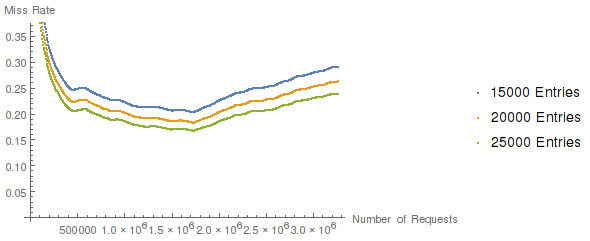
\includegraphics[scale=.4]{graph.png}
\caption{Number of Requests vs. Miss Rate}
\end{figure}

\begin{figure}[h!]
\centering
\begin{tabular}{l|r|r|r}
&15k&20k&25k\\\hline
Hit Rate& 71\% & 74.8\% & 76.1\%
\end{tabular}
\caption{The overall hit rate at each cache size.}
\end{figure}

Figure 4 contains the hit rates produced by the different cache sizes.
As expected, the hit rate monotonically increases with the cache size.

\section{Experimental Framework}

The test was run on a machine running Arch Linux with the kernel \verb|4.2-ck| with an Intel i7-4770k quad-core processor with eight threads at 4.2GHz and 16GB of DDR3 1333MHz RAM.
The executables, the id list, and web server trace file were stored on a SSD and all directories and databases were written to a 5400RPM mechanical harddrive mounted at \verb|./ext|.
The mechanical harddrive was filled with a single EXT2 partition.

The code we used to run our tests can be found at \url{https://github.com/matt-mccarthy/verdant-octo-kumquat}.
We wrote all code for the tests in C++ with \verb|g++-5.2.0| as the compiler with the \verb|-O3| flag enabled.
Furthermore, we utilized Boost to provide a C++ \verb|mmap| wrapper.
We wrote a shell script named \verb|run.sh|that managed our test parameters and invoked our \verb|db-gen| to create the directory and database.
Afterwards, \verb|run.sh| ran the \verb|benchmark| program in its various modes in order to gather the results.

The usage of \verb|run.sh| is:\\
\begin{footnotesize}
\verb|run.sh <trace> <modulus> <file size> <num trials>|\\
\verb|<cache line> <number of lines>|
\end{footnotesize}\\
For our tests, we ran,\\
\begin{footnotesize}
\verb|run.sh trace.txt 250 14336 5 1 <Cache Size>|
\end{footnotesize}\\
\section{Future Work}

Since our cache only exploited temporal locality, one could add prefetching to the cache in order to improve the hit rate by exploiting spacial locality.
Furthermore, one could lower the overhead of the cache to improve read performance.
Another interesting improvement would be to add multithreaded prefetching to see if any performance gains can be achieved.

\section{Conclusion}

As the data suggests, locality is a powerful tool at our disposal which can easily improve performance of disk I/O bound applications.
By adding a simple cache with a least recently used replacement policy, we reduced the execution time of our toy database reader by 25\% of the original exectution time.
Furthermore, in order to get a hit rate within 20\% of the maximal hit rate, we only need to store 350MB of our 2GB database in memory, thus leaving us more resources for other tasks.

\printbibliography

\end{document}
